\jrnlday{Bonne nouvelle d'une grande joie}


\dvepigraph{%
Mais l’ange leur dit≡ Soyez sans crainte, car je vous annonce la bonne nouvelle d’une grande joie qui sera pour tout le peuple […] Et soudain il se joignit à l'ange une multitude de l'armée céleste, qui louait Dieu et disait≡ Gloire à Dieu dans les lieux très hauts, et paix sur la terre parmi les hommes qu'il~agrée!}{\ibibleverse{Lc}(2:10,13,14)}

En cette période de l'année, c'est vraiment merveilleux d'entendre les paroles \og pleines de Christ \fg{} de cantiques comme \emph{Le Monde en Joie}, \emph{Ô Peuple Fidèle}, \emph{Écoutez le Chant des Anges} qui sont joués jusque dans les centres commerciaux quand nous faisons nos achats de Noël.

Les cantiques sur la naissance de Jésus ont littéralement transformé Noël dans l'Angleterre du XVII\up{e} siècle. Les fêtes d'hiver étaient devenues tellement tumultueuses avec de l'ivrognerie et des émeutes, que les honnêtes gens avaient peur de sortir et que le Parlement Anglais avait dû passer une loi interdisant la célébration de Noël.

Petit à petit, les chants de Noël parlant de Jésus ont commencé à devenir populaires et beaucoup de gens ont commencé à célébrer Noël avec des chants d'adoration et de louange. Noël est redevenu légal – une autre bonne raison pour garder Christ dans Noël.

Quand l'ange a chanté le tout premier chant de Noël aux bergers, il a dit≡ \og Je vous annonce la bonne nouvelle d’une grande joie qui sera pour tout le peuple. \fg{} Le mot \og joie \fg{} est \emph{chara} en grec, qui signifie \og gaieté et délices \fg{} et qui est la racine du mot \emph{charis}, l'étonnante grâce de Dieu. En nous donnant Christ, Dieu nous a donné Sa grâce indicible, Son amour et ses bénédictions non mérités. C'est le cadeau le plus joyeux que nous puissions recevoir.

Les anges ont annoncé aux bergers la \og bonne nouvelle d'une grande joie \fg{} (\ibibleverse{Lc}(2:10)), littéralement d'une \og méga joie \fg{}, et quand les mages ont vu l'étoile, \og ils éprouvèrent une très grande joie \fg{} (\ibibleverse{Mt}(2:10)). Autrement dit, les mages \og tremblaient violemment en proie à des frissons de joie! \fg{}

Aujourd'hui, notre monde recherche désespérément la joie. Nous voulons être joyeux et insouciants parce que nous vivons au milieu de tant de pression, de stress et de situations pesantes. Nous pensons souvent que la joie vient d'avoir davantage d'argent, mais si c'était vrai Donald Trump serait un modèle de joie.

Le philosophe Sénèque a donné un jour le conseil suivant≡ \og Pour être heureux, n'ajoutez pas à vos possessions, mais soustrayez à vos désirs. \fg{} Il est très probable notre poursuite des richesses est la mauvaise herbe qui tue en l'étouffant une relation joyeuse avec Dieu.

% Image helps moving on to next page
\mbox{}\hfill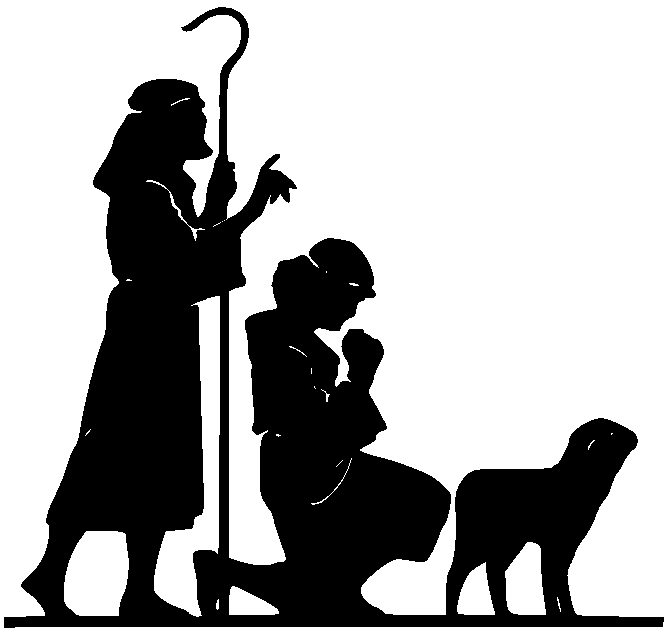
\includegraphics[height=4cm]{images/nativity.pdf}\hfill\mbox{}

Jésus nous a dit de débarrasser nos cœurs de ces mauvaises herbes qui nous volent du temps car elles nous gardent loin de Lui. Ce Noël, rappelez-vous que la vraie joie ne vient pas des choses matérielles, mais qu'elle vient d'une profonde et tendre relation avec Jésus.
\nopagebreak

\dvquote{%
Vous l’aimez sans l’avoir vu. Sans le voir encore, vous croyez en lui et vous tressaillez d’une allégresse indicible et glorieuse, en remportant pour prix de votre foi le salut de vos âmes.}{\ibibleverse{IP}(1:8-9)}

\ornrule

\dvquote{%
Puis il leur dit≡ Gardez-vous attentivement de toute cupidité; car même dans l’abondance, la vie d’un homme ne dépend pas de ce qu’il possède.}{\ibibleverse{Lc}(12:15)}

